\documentclass[a4paper,11pt]{article}

\input ../include/preamble.tex

% Finite state machines
\usepackage{tikz}
\usetikzlibrary{automata,arrows,topaths}


% SECTIONS
%
% * Introduction
% * A chopstick
% * A philosopher
% * Dinner at the table
% * Experiments
% * Break the deadlock
% * Asynchronous requests
% * A waiter
% * Benchmark
% * Avoid the deadlock


\begin{document}

% ================================================== %
% == Title  == %
% ================================================== %

\title{
    \textbf{Philosophers and Concurrency}\\
    \large{Programming II - Elixir Version}
}
\author{Johan Montelius}
\date{Spring Term 2018}
\maketitle
\defaultpagestyle


% ================================================== %
% == Introduction  == %
% ================================================== %

\section*{Introduction}

In this assignment you should implement the behavior of five
philosophers that are sitting at a round dining table. The problem is to
allow each philosopher to get something to eat, a task that does not
sound to be very difficult. 

The situation is that the five philosophers are sitting at the dinner
table with a bowl of noodles in front of them, and a chopstick
between each of them. We thus have five philosophers and only five
chopsticks, this is the problem.

When a philosopher decides to eat (they sit and think most of the
time), she will pick up the two chopsticks next to her and eat from
the bowl of noodles. When she is done, she will simply return the
chopsticks to their places. If the philosophers do not eat that often
things will probably work out just fine, the problem occurs when
several philosophers decide to eat at the same time.

You should complete a simple program that implements the behavior
of the philosophers and run some experiments to see when things go
wrong. You should also provide a solution to the problem that at least
allow some of the philosophers to get some food.  


% ================================================== %
% == A chopstick  == %
% ================================================== %

\section{A chopstick}

The location of a chopstick is represented by a process. The state of
the process is either:

\begin{itemize}
\item {\tt available} : if a chopstick is present or,
\item {\tt gone} : if the chopstick is taken
\end{itemize}

A location will start in the state available, and then wait for a {\em request message}. When the location process receives this message it
should return a {\em granted} message and move to the state {\em gone}.
In this state the location process will accept a {\em return message} 
and can then return to the available state. Messages that are not currently handled remain in the message queue.

\begin{figure}[h!]
    \centering
    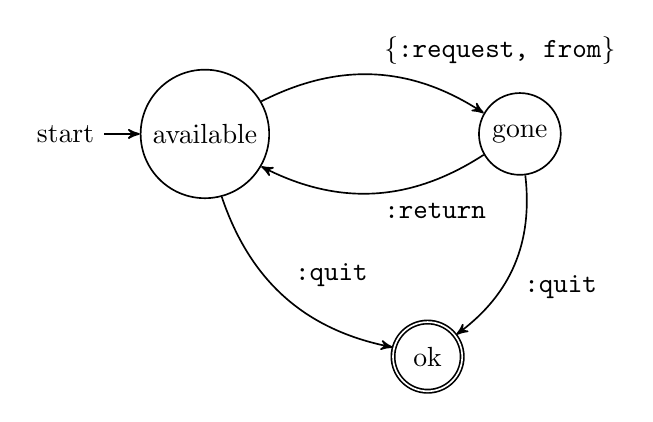
\begin{tikzpicture}[>=stealth', node distance=4cm, semithick, auto]
        \node[initial, state]            (av)                           {available};
        \node[state]                     (go)         [right of=av]     {gone};
        \node[accepting, state]          (te)   [below right of=av]     {ok};
    
        \path[->]   (av) edge       [bend left]    node      {{\tt \{:request, from\}}}    (go)
                          edge       [bend right]   node      {{\tt :quit}}                 (te);
        \path[->]   (go) edge       [bend left]    node      {{\tt :return}}               (av)
                          edge       [bend left]    node      {{\tt :quit}}                 (te);
    \end{tikzpicture}
\end{figure}

Implement this process in a module {\tt Chopstick} with a
function {\tt start/0} that spawns the process and returns the process
id. When you spawn the process use {\tt spawn\_link/1} to make sure
that the chopstick process dies if the mother process dies (and vice
verse). This is some skeleton code to give you the structure of the
implementation.

\begin{minted}{elixir}
def start do
  stick = spawn_link(fn -> ... end)
end

def available() do
  receive do
    ... -> ...
    :quit -> :ok
  end
end

def gone() do
  receive do
    ... -> ...
    :quit -> :ok
  end
end
\end{minted}

We should try to keep the internals of the location process as hidden
as possible from the users of the module. We therefore provide a
functional interface so that a user of the module does not need to
know the structure of all messages.

\begin{minted}{elixir}
def request(stick) do
  send(stick, ...)
  receive do
    ... -> :ok
  end
end
\end{minted}

Provide similar functions for returning the stick and terminating the
process. We will change things later so you will see that it is very
nice to only allow the philosophers to use the functional interface.


% ================================================== %
% == A philosopher  == %
% ================================================== %

\section{A philosopher}

A philosopher is either dreaming (some call it thinking), waiting for
a chopstick or eating. In the dreaming state the philosopher does
nothing until she decides that it is time to eat. She will then
request her left chopstick and her right chopstick, if everything
works she can start to eat. A philosopher will eat for while and then
return the chopsticks.

You can implement the dreaming and eating time by using the library
function {\tt :timer.sleep/1} that will simply wait for a number of
milliseconds before continuing. If you want to have some randomness
you can use the library function {\tt :rand.uniform/1}. This sequence
will make a process sleep for a random time.

\begin{minted}{elixir}
def sleep(0) do :ok end
def sleep(t) do 
  :timer.sleep(:rand.uniform(t))
end
\end{minted}

Implement the philosopher in a module called {\tt Philosopher} and
provide a function {\tt start/5} that spawns a philosopher
process (use spawn\_link/1). The procedure should take the following arguments.

\begin{itemize}

\item {\tt hunger}: the number of times the Philosopher should eat
  before it sends a {\tt :done} message to the controller process.

\item {\tt right} and {\tt left}: the process identifiers of the two
  chopsticks.

\item {\tt name}: a string that is the name of the philosopher, used
  for nice logging.

\item {\tt ctrl}: a controller process that should be informed when
  the philosopher is done.
\end{itemize}

Add some nice logging information to your process so that you can
track what is happening. A philosopher could for example print a
message when it receives a chopstick:

\begin{minted}{elixir}
IO.puts("#{name} received a chopstick!")
\end{minted}

Elixir also supports string interpolation; in the code fragment above
the content of the variable {\tt name} is interpolated with the rest
of the string.


% ================================================== %
% == Dinner at the table  == %
% ================================================== %

\section{Dinner at the table}

If you have the two modules working we can seat the philosophers
around the table. We first create the locations and then start the
philosophers. In a module called {\tt Dinner}, define the following
function:

\begin{minted}{elixir}
def start(), do: spawn(fn -> init() end)

def init() do
  c1 = Chopstick.start()    
  c2 = Chopstick.start()
  c3 = Chopstick.start()
  c4 = Chopstick.start()
  c5 = Chopstick.start()
  ctrl = self()
  Philosopher.start(5, c1, c2, "Arendt", ctrl)
  Philosopher.start(5, c2, c3, "Hypatia", ctrl)
  Philosopher.start(5, c3, c4, "Simone", ctrl)
  Philosopher.start(5, c4, c5, "Elisabeth", ctrl)
  Philosopher.start(5, c5, c1, "Ayn", ctrl)
  wait(5, [c1, c2, c3, c4, c5])
end
\end{minted}

We're starting all processes under a controlling process that will keep
track of all the philosophers and also make sure that the chopstick
processes are terminated when we're done.

\begin{minted}{elixir}
def wait(0, chopsticks) do
  Enum.each(chopsticks, fn(c) -> Chopstick.quit(c) end)
end
def wait(n, chopsticks) do
  receive do
    :done ->
      wait(n - 1, chopsticks)
    :abort ->
      Process.exit(self(), :kill)
  end
end
\end{minted}

If things go wrong and a process terminates with an error it will kill
all linked processes. If things are stuck in a deadlock we can send
an {\tt :abort} message to the controller process that then will exit
with an error and kill all other processes.

Now it's time to see if the philosophers will be able to dream and eat. 


% ================================================== %
% == Experiments  == %
% ================================================== %

\section{Experiments}

Experiment with the dinner, will the philosophers always be able to
eat? What happens if you decrease the time it dreams? What happens if
you introduce an artificial delay between the receiving of the first
chopstick and requesting the second?


% ================================================== %
% == Break the deadlock  == %
% ================================================== %

\section{Break the deadlock}

To break out of a potential deadlock situation we can change the
request function in the chopstick module. Let's pass a second argument
to the function that specifies how many millisecond we are willing to
wait for a chopstick.

\pagebreak

\begin{minted}{elixir}
def request(stick, timeout) do
  send(stick, ...)
  receive do
    ... -> 
      :ok
  after ... -> 
    :no
  end
end
\end{minted}

Change your implementation of the philosophers to use the new
interface. At this time it is worth understanding a bit about the
random module. It will as you have figured out generate a random
number each time we can {\tt :rand.uniform/1} but, the sequence is 
the same each
time we create a new process. A process will use the same sequence
every time it is created. This is very nice when we debug programs
since we then eliminate one source of indeterminism, but not as fun
when we want processes to behave different each time we run it. Do
some reading and provide each philosopher with a unique seed value, if
you do it right you can have different execution patterns at will.

So you have broken the dead-lock, or so you think, but what is
actually happening? What happens when a philosopher gives up? You have
to do some thinking but the solution is quite simple once you trace
what is happening.


% ================================================== %
% == Asynchronous requests  == %
% ================================================== %

\section{Asynchronous requests}

The solution that you have now is quite boring in that a philosopher
will first request the left chopstick and only when this is delivered
will it try to grab the right chopstick. How about sending a request
to both chopsticks first and then wait for the replies? Change the
request function and then provide a {\em granted} function that does
the waiting. 

If a philosopher gives up, how do we keep track of which chopsticks
that was actually obtained? Is this a tricky problem or a non-problem?


% ================================================== %
% == A waiter  == %
% ================================================== %

\section{A waiter}

Can you provide a better strategy for the philosophers so that they
can eat and dream without ending up in a deadlock? What happens if
you provide a waiter that controls how many philosophers that can eat
at any given time. How would this help the situation? How many
philosophers can try to eat without ending up in a deadlock? How
smart does the waiter need to be?


% ================================================== %
% == Benchmark  == %
% ================================================== %

\section{Benchmark}

Run some benchmarks and try to figure out how long time it takes for a
set of philosophers to eat a given number of times. Use the algorithms
that do not risk ending up in deadlocks and try to be as aggressive as
possible.  

Can you work with a increasing ``back-off'' time so that a philosopher
will wait for a while before trying to grab the chopsticks if it has
failed once? Can the system adapt itself so that it runs smoothly
without too many failed attempts? Is there a trade-off between being
aggressive and over-all throughput?


% ================================================== %
% == Avoid the deadlock  == %
% ================================================== %

\section{Avoid the deadlock}

Is there a small change in the system that will avoid ever landing in
a dead-lock situation? Can you guarantee that all philosophers will
eventually get to eat? Is the system fair?

\end{document}
